\chapter{Testes e Resultados}
\label{ch::testes}

%\section{Introdução}
%\label{sec::testes:intro}

Durante a implementação e após a conclusão da versão final do projeto \theapp, foram realizados diversos testes a fim de analisar a exatidão do algoritmo e a qualidade das renderizações obtidas. O presente Capítulo explora os testes e respetivos resultados obtidos no sistema de renderização com aceleração por \textit{hardware}. Em último será feita uma menção à renderização por \textit{software}.

Doravante, referir-se-á ao programa final exclusivamente pelo seu nome, \theapp. Deve ainda ser assumido que, em toda a sequência de testes feita e registada, a aplicação foi compilada em \textbf{modo \textit{debug}} (no qual o programa retorna informação detalhada útil neste processo).


\section{Arranque e \textit{Setup} Inicial}
\label{sec::testes::start}

A \theapp~permite modular o seu comportamento através de argumentos passados por linha de comandos. Este é o passo de \textit{setup} inicial do programa.

\begin{itemize}
	\item \verb|-r| (\textit{render mode}): permite definir qual o motor de renderização a ser usado. As opções são:
	\begin{itemize}[nosep]
		\item \verb|CPU|: motor de renderização por \textit{software} (faz usufruto da \ac{CPU});
		\item \verb|GPU|: aceleração por \textit{hardware} (com recurso à \ac{GPU}).
	\end{itemize}
	
	\item \verb|-t| (\textit{threads}): permite definir o número de \textit{threads} a serem usadas no motor de renderização por \textit{software}. Por defeito irá utilizar metade dos núcleos lógicos disponíveis. Caso o utilizador defina um número superior, um aviso é emitido sobre a potencial perda de \textit{performance}.
\end{itemize}

O programa irá carregar todos os recursos necessários ao seu bom funcionamento, em particular:
\begin{itemize}
	\item Bibliotecas e \textit{frameworks} (GLFW e \acs{GLAD});
	\item \textit{Shaders} para texto, logótipo e superfície implícita;
	\item Fonte para o texto e imagem do logótipo.
\end{itemize}

Em caso de erro, o programa não arranca e a sua execução é abortada. Em caso de sucesso, é apresentada uma janela com a \textit{home screen} do programa (Figura \ref{fig::home}). O utilizador pode selecionar o ficheiro com as funções a renderizar pressionando a tecla \verb|O|.

\begin{figure}[!htbp]
	\centering
	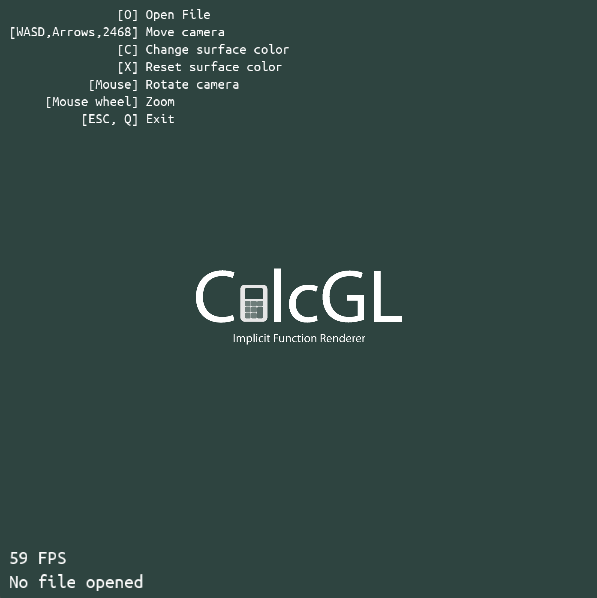
\includegraphics[width=.8\textwidth]{home}
	\caption[Ecrã inicial da aplicação]{Ecrã inicial da aplicação \theapp.}
	\label{fig::home}
\end{figure}


\section{Testes com Funções Implícitas Conhecidas}
\label{sec::testes:dev}

A fase de desenvolvimento para o sistema de aceleração por \textit{hardware} englobou duas fases distintas:
\begin{enumerate}
	\item Declaração das funções implícitas em código \acs{GLSL} de forma direta no \textit{fragment shader};
	\item Injeção das funções implícitas lidas a partir de ficheiros externos.
\end{enumerate}

A primeira fase foi fundamental para limar a implementação do algoritmo e fazer prova de conceito do uso exclusivo do \textit{fragment shader}. A primeira renderização feita com sucesso foi uma esfera colorida a verde e com sombra (Figura \ref{fig::calcglsphere}), numa tentativa de replicar o resultado obtido no \textit{website} \url{shadertoy.com} (Figura \ref{fig::ashalgosphere}) com recurso ao \textbf{algoritmo naïve}.

\begin{figure}[!htbp]
	\centering
	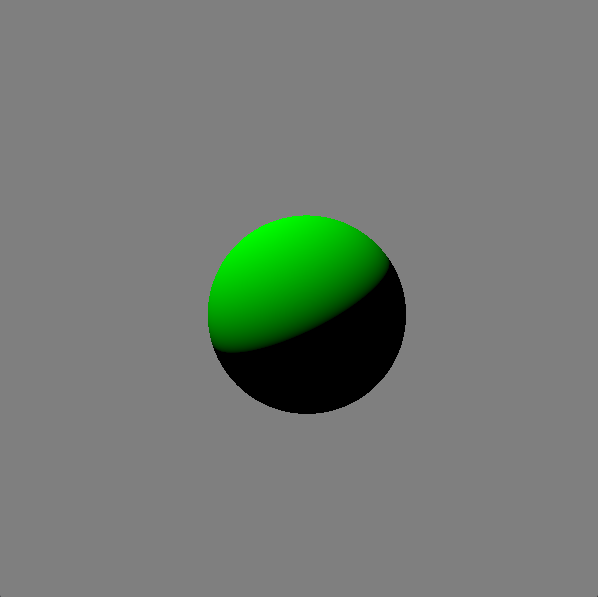
\includegraphics[width=.7\textwidth]{calcglsphere}
	\caption[Esfera no \theapp~com algoritmo naïve]{Esfera renderizada no \theapp, em fase inicial de testes, com o algoritmo naïve.}
	\label{fig::calcglsphere}
\end{figure}

O \textit{fragment shader} que produziu este resultado foi então adaptado para mostrar nove sólidos cujas \acfp{SDF} são bem conhecidas, em conjunto com um plano e dois pontos de luz para conferir o devido funcionamento das sombras. Uma vez que as \acsp{SDF} são conhecidas, foi utilizado o algoritmo de \textbf{\itshape sphere tracing}. O resultado obtido consta da Figura \ref{fig::sphereoriginalblue}.

Por fim, o \textbf{parâmetro de suavização} $s$ (equação (\ref{eq::suavizacao})) foi testado em função do tempo $t$ tal que $s = \cos(t)$; na Figura \ref{fig::spheresmooth} é apresentada uma \textit{frame} do resultado obtido.

De notar que, em todos os testes com o algoritmo \textit{sphere tracing}, o programa executou à taxa de frequência do monitor (60 ou 75 \acf{fps}).

\begin{figure}[!htbp]
	\centering
	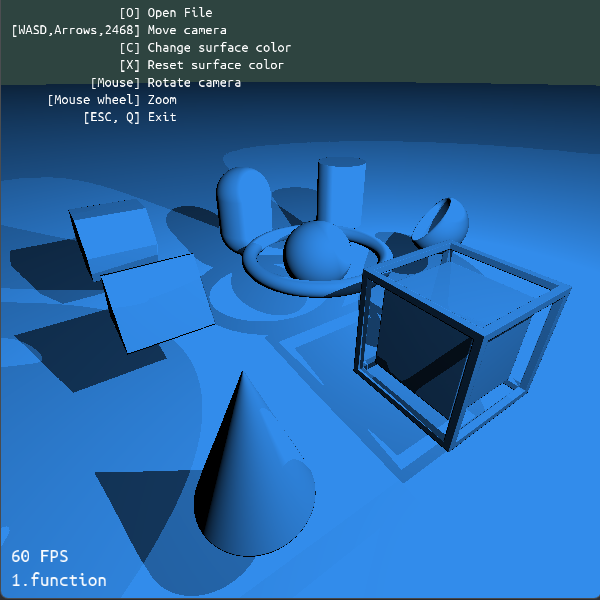
\includegraphics[width=.8\textwidth]{sphereoriginalblue}
	\caption[Nove objetos com \textit{sphere tracing} no \theapp]{Renderização de nove objetos no \theapp~usando o algoritmo de \textit{sphere tracing}.}
	\label{fig::sphereoriginalblue}
\end{figure}

\begin{figure}[!htbp]
	\centering
	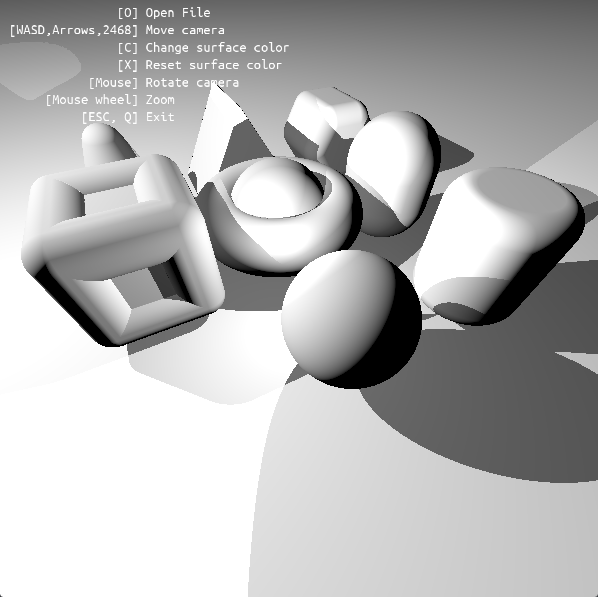
\includegraphics[width=.8\textwidth]{spheresmooth}
	\caption[Nove objetos com \textit{sphere tracing} e suavização no \theapp]{Renderização de nove objetos no \theapp~usando o algoritmo de \textit{sphere tracing} com um fator de suavização $s$ dependente do tempo de execução $t$, em particular $s = \cos(t)$.}
	\label{fig::spheresmooth}
\end{figure}


\section{Resultados para Funções Implícitas Arbitrárias}
\label{sec::testes:resultados}

Após o funcionamento de ambos os algoritmos naïve e \textit{sphere tracing} ter sido demonstrado com sucesso, procedeu-se aos testes finais a fim de alcançar o objetivo principal do projeto. Para tal, foram utilizadas as seguintes condições:

\begin{itemize}
	\item \textbf{Algoritmo}: naïve (uma vez que as \acsp{SDF} não são conhecidas);
	\item \textbf{Funções implícitas}: fornecidas por ficheiros externos;
	\item \textbf{\itshape Fragment shader}: recompilado em \textit{runtime} para que as funções implícitas lhe sejam injetadas.
\end{itemize}


Dos testes realizados, três funções implícitas em particular são apresentadas:

\begin{enumerate}
	\item \textbf{Superfície $\Pi$} (Figura \ref{fig::calcglpisurf}), dada pela expressão:
	\begin{align*}
		f(x,y,z) = ~& \left(x^2 + y^2 + z^2 - 1\right) \times \\
	                & \left((x-2)^2 + (y-1)^2 + z^2 - 1\right) \times \\
		            & \left((x-1)^2 + (y-2)^2 + (z-2)^2 - 1\right) - 5
	\end{align*}

	\item \textbf{\textit{Genus}} (Figura \ref{fig::calcglgenus}), dado pela expressão:
	\begin{equation*}
		f(x,y,z) = 2y(y^2 - 3x^2)(1-z^2) + (x^2 + y^2)^2 - (9z^2 - 1)(1 - z^2)
	\end{equation*}

	\item \textbf{Fractal} (Figura \ref{fig::calcglfractal}), dado pela expressão:
	\begin{align*}
		f(x,y,z) =~ & (x^3 - 3xy^2 - 3xz^2)^2 + (y^3 - 3x^2y - 3yz^2)^2 + \\
		            & (z^3 - 3x^2z + y^2z)^2  - (x^2 + y^2 + z^2)^3
	\end{align*}
\end{enumerate}

Pode-se constatar que o algoritmo implementado perde bastante detalhe com um fractal devido às limitações impostas a nível de cálculo. Uma maior precisão seria necessária, mas tal levaria a uma execução bastante pobre por parte da aplicação com o algoritmo naïve (conforme discutido na Secção \todo{Secção que fala sobre a GPU dar reset}).

\begin{figure}[!htbp]
	\centering
	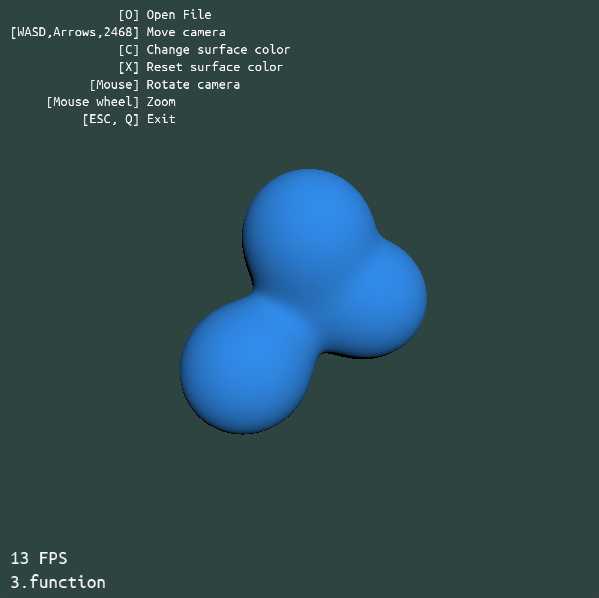
\includegraphics[width=.8\textwidth]{calcglpisurf}
	\caption[Superfície $\Pi$ no \theapp~com algoritmo naïve]{Superfície $\Pi$ renderizada no \theapp~com algoritmo naïve.}
	\label{fig::calcglpisurf}
\end{figure}

\begin{figure}[!hbp]
	\centering
	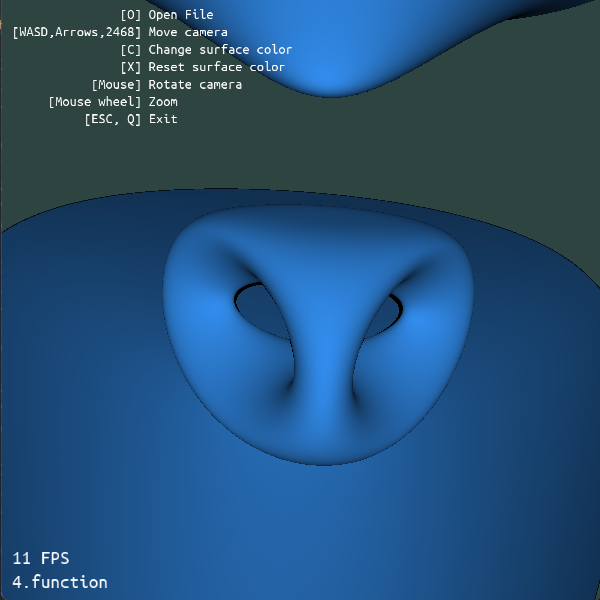
\includegraphics[width=.8\textwidth]{calcglgenus}
	\caption[\textit{Genus} no \theapp~com algoritmo naïve]{\textit{Genus} renderizado no \theapp~com algoritmo naïve.}
	\label{fig::calcglgenus}
\end{figure}

\begin{figure}[!hbp]
	\centering
	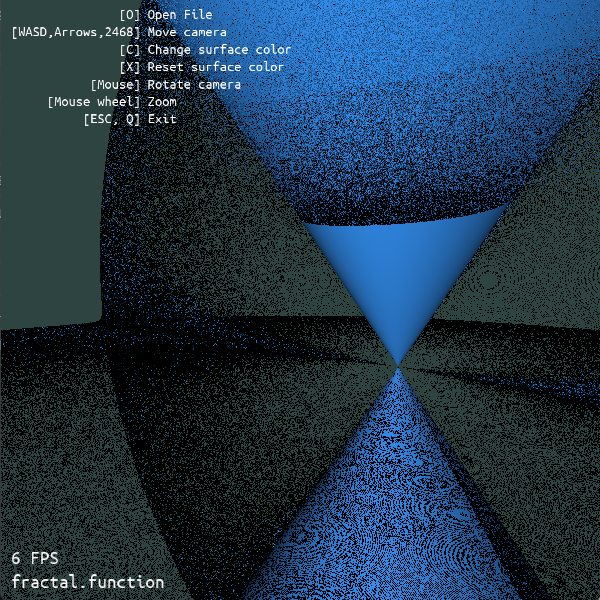
\includegraphics[width=.7\textwidth]{calcglfractal}
	\caption[Fractal no \theapp~com algoritmo naïve]{Fractal renderizado no \theapp~com algoritmo naïve.}
	\label{fig::calcglfractal}
\end{figure}



\section{Renderização por \textit{Software}}
\label{sec::testes:software}

A renderização por \textit{software} (i.e. com recurso exclusivo à \ac{CPU}) revelou-se extremamente ineficiente, sendo impraticável. Não obstante, a paralelização em \textit{threads} foi testada a fim de verificar os tempos de execução para uma única \textit{frame}. O tempo foi contabilizado pela própria aplicação.

Não só devido ao tempo de execução, mas também por exigir bastante da \ac{CPU}, apenas foram testados quatro cenários no computador \textit{desktop} da Tabela \ref{tab::hardware}. O tempo mínimo de execução foi alcançado com 2 \textit{threads}, num tempo aproximado de 1 hora e 40 minutos. Um maior número de \textit{threads} revelou ser prejudicial à \textit{performance}. Estes tempos estão sumariados na Tabela \ref{tab::render_cpu} e no gráfico da Figura \ref{fig::cpurenderchart}.

\begin{table}[!hbtp]
	\centering
	\caption[Tempos de renderização em \acs{CPU}]{Tempo para a renderização de uma única \textit{frame} com recurso à \acs{CPU} para diferentes números de \textit{threads}. O tempo em segundos foi arredondado à unidade.}
	\label{tab::render_cpu}
	\begin{tabular}{r r r}
		\toprule
		\multirow{2}{*}{\textbf{Threads}} & \multicolumn{2}{c}{\textbf{Tempo}} \\
		\cline{2-3}
		& Segundos & h:m's'' \\
		\midrule
		1 &  7087 & 01:58'07'' \\
		2 &  5984 & 01:39'44'' \\
		4 &  7566 & 02:06'06'' \\
		6 & 10414 & 02:53'34'' \\
		\bottomrule
	\end{tabular}
\end{table}

\begin{figure}[!hbtp]
	\centering
	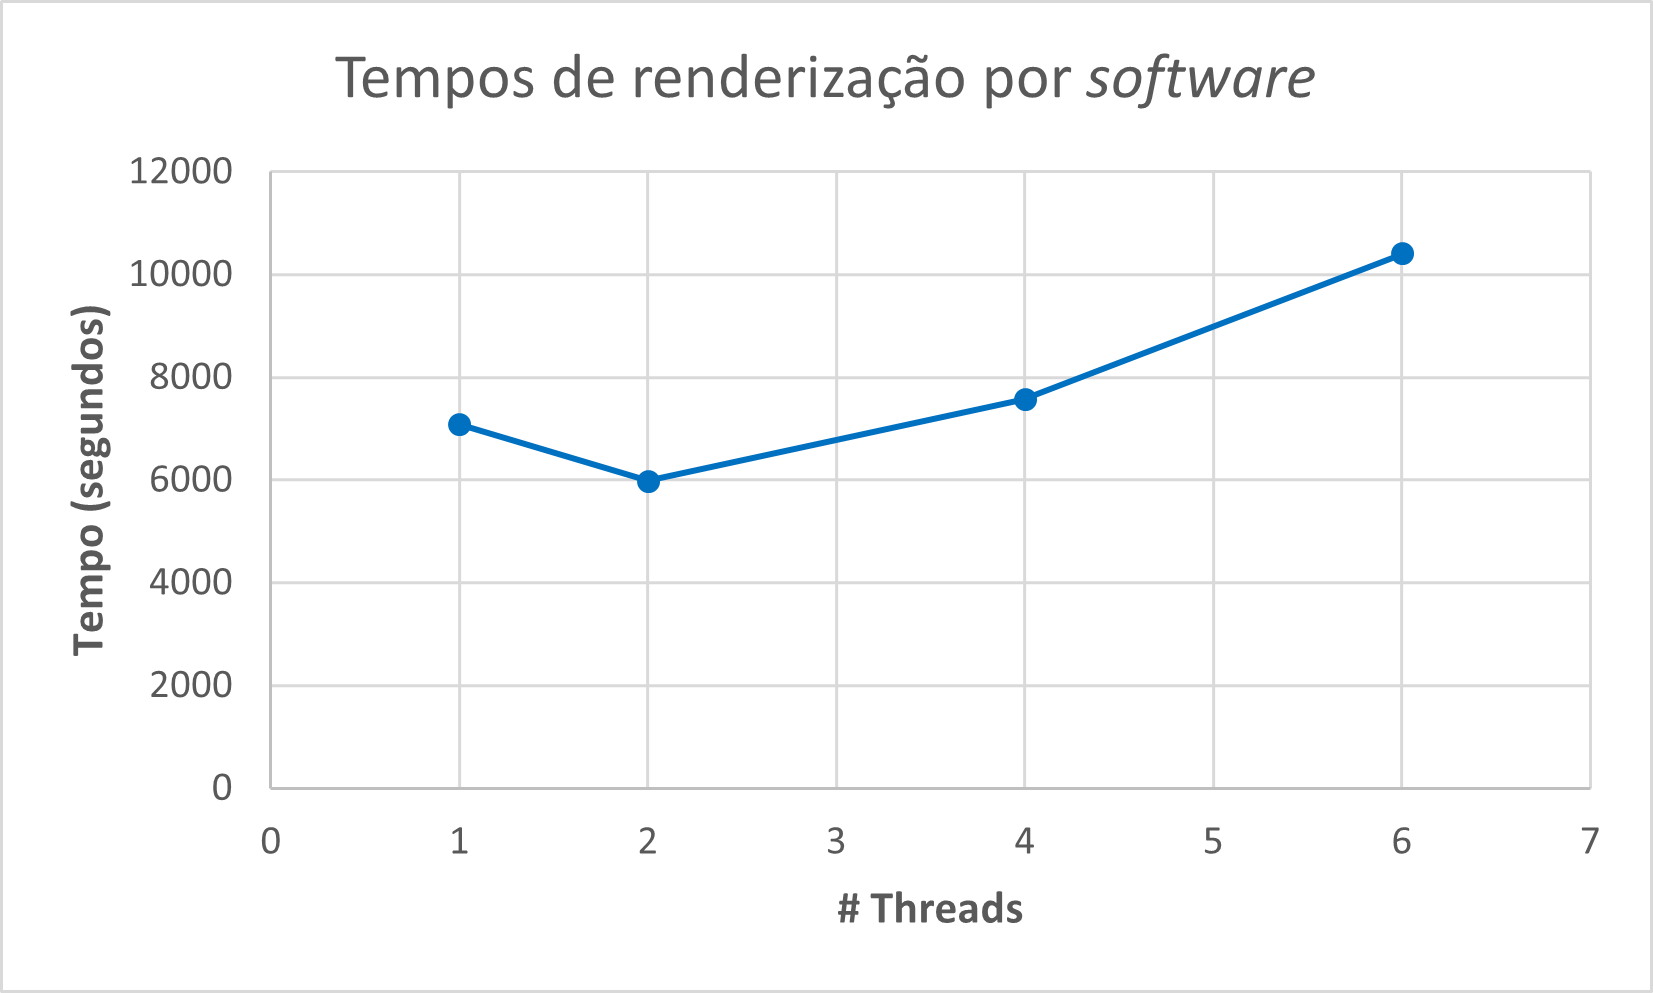
\includegraphics[scale=0.9]{cpurenderchart}
	\caption[Gráfico dos tempos de execução em \acs{CPU}]{Gráfico representativo dos tempos de execução em \acs{CPU}, correlacionando o número de \textit{threads} com o tempo em segundos para concluir uma \textit{frame}.}
	\label{fig::cpurenderchart}
\end{figure}
